\documentclass[12pt]{article}
\usepackage[utf8x]{inputenc}
\usepackage[english,russian]{babel}
\usepackage[section]{placeins}
\usepackage{upgreek}
\usepackage{graphicx}
\usepackage[left=3cm, right=1.5cm, top=2cm, bottom=2cm]{geometry}
\usepackage{caption}
\usepackage{subcaption}
\usepackage{indentfirst}
\usepackage{wrapfig}
\usepackage{amsmath}
\usepackage{gensymb}
\usepackage{setspace}
\usepackage{placeins}
\graphicspath{{images/}}

\begin{document}

\title{Коэффициент дилюции для горячего аккреционного пятна}
\date{}
\maketitle

По определению, коэффициент дилюции равен 

\begin{equation}\label{eq:dilut-def}
W = \frac{\Omega}{4\pi},
\end{equation}
и для его вычисления необходимо найти телесный угол излучающей области: $\Omega$. В случае магнитосферного аккреционного пятна она представляет собой две полосы ограниченными двумя параллелями на поверхности звезды. Границы этих полос можно найти из уравнения линий дипольного магнитного поля:

\begin{equation}\label{eq:dip-line}
r = r_\text{m} \sin(\theta),
\end{equation}   
где $\theta$ --- полярный угол. Тогда, предположив, что магнитосфера ограничена двумя линиями поля с $r_\text{m} = r_\text{o}$ и $r_\text{m} = r_\text{i}$, можно найти границы аккреционного пятна, положив в уравнении~\eqref{eq:dip-line} $r = R_\star = 1$:

\begin{equation}\label{eq:star-field}
\begin{aligned}
\varphi_{11} &\le \varphi_1 \le \varphi_{12}, \\
\varphi_{22} &\le \varphi_2 \le \varphi_{21}, \\
\varphi_{11,21}& = \arcsin(\pm\sqrt{r_\text{o}^{-1}}), \\
\varphi_{12,22}& = \arcsin(\pm\sqrt{r_\text{i}^{-1}}), 
\end{aligned}
\end{equation}
где $\varphi_{11,12}$ ограничивают одну полосу, а $\varphi_{21,22}$ --- вторую. 

В общем виде можно записать, что

\begin{equation}\label{eq:omega-def}
\Omega = \int\limits_{(\Omega_\text{o})} \text{d}\Omega',
\end{equation}
где $(\Omega_\text{o})$ --- вид области из точки в магнитосфере, в которой мы считаем дилюцию. Так как область удобно записывается относительно центра звезды, то логично перейти к интегрированию по ее поверхности. Сделаем это при помощи рис. \ref{fig:transition}. Очевидно, что элемент площади области $\text{d}S' = \cos(\alpha)\text{d}S$, а следовательно

\begin{equation}\label{eq:transition}
\text{d}S' = r'^2\text{d}\Omega' = \cos(\alpha)\text{d}S = \cos(\alpha)\text{d}\Omega \Rightarrow \text{d}\Omega' = \frac{\cos(\alpha)}{r'^2}\text{d}\Omega,
\end{equation}
так как область находится на поверхности звезды, а ее радиус равен единице. Подставляя \eqref{eq:transition} в \eqref{eq:omega-def} и \eqref{eq:dilut-def} получаем 

\begin{equation}\label{eq:dilut-star}
W = \frac{1}{4\pi}\int\limits_{(\Omega_\star)}\frac{\cos(\alpha)}{r'^2}\text{d}\Omega
\end{equation}

\begin{figure}[h]
\centering
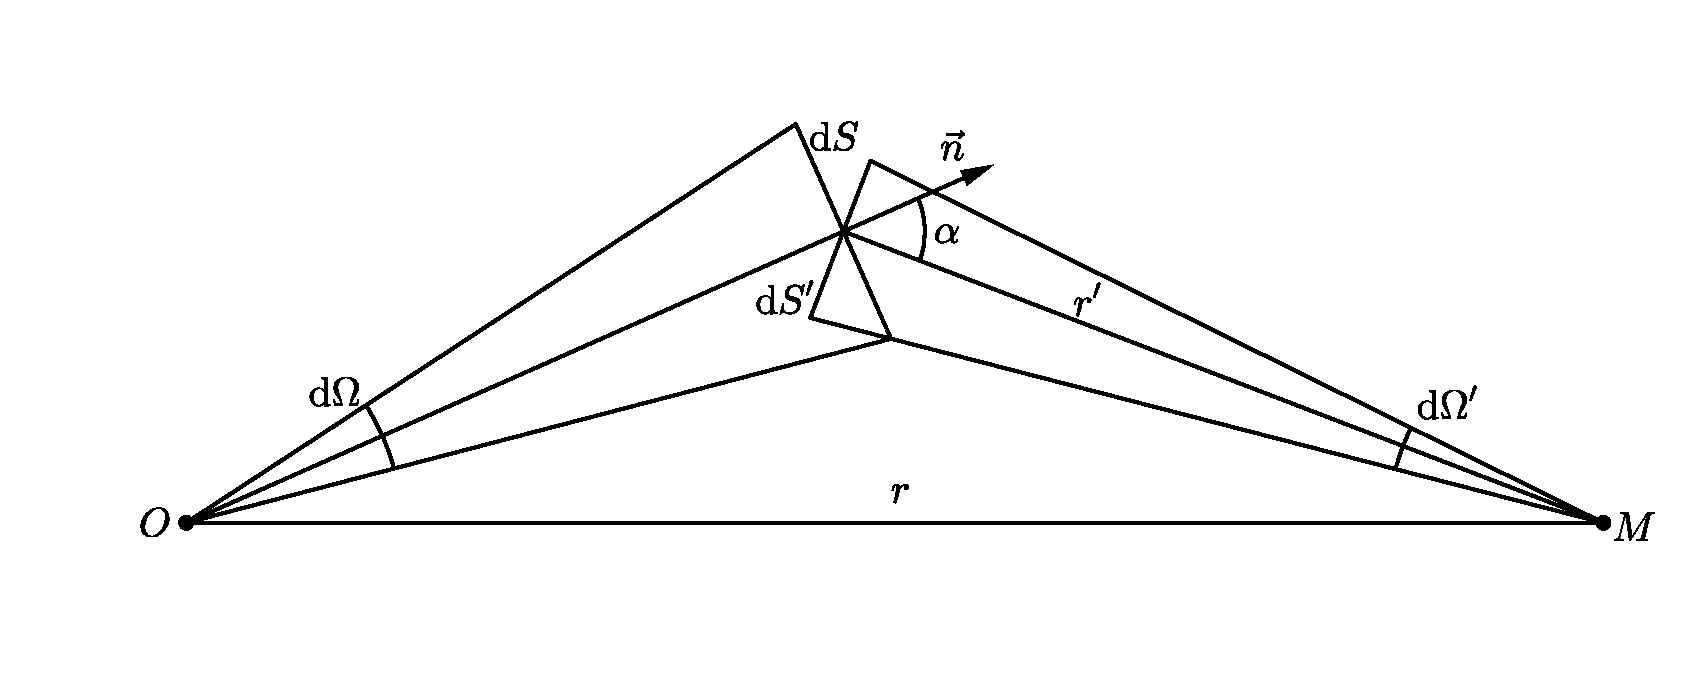
\includegraphics[width=\textwidth]{dilut.eps}
\caption{Переход от системы отсчета точки M, в которой рассчитывается дилюция, к звезде (точка O)}
\label{fig:transition}
\end{figure}

\begin{figure}[h]
\centering
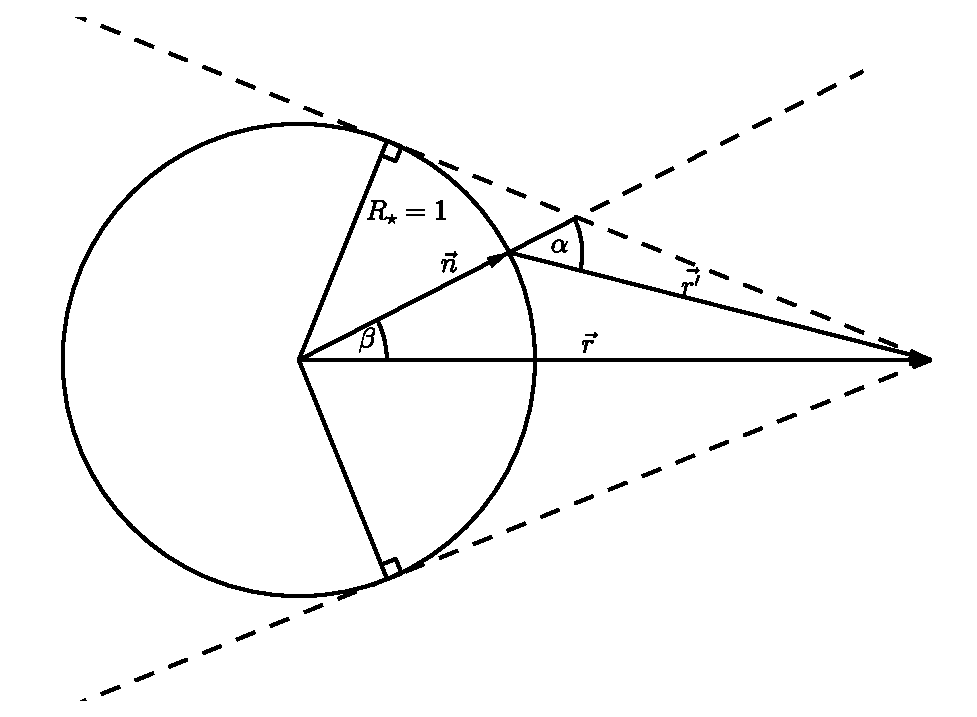
\includegraphics[width=0.6\textwidth]{view.eps}
\caption{Вид на поверхность звезды и точку $\vec{n}$ на ней из точки $\vec{r}$}
\label{fig:star-view}
\end{figure}

Теперь нужно выразить видимую из точки в магнитосфере область звезды в координатах на ее поверхности. Для этого рассмотрим вектор $\vec{n}$, указывающий из центра звезды в точку на ее поверхности, и вектор $\vec{r}$ --- вектор, указывающий в направлении на точку в магнитосфере. Как видно из рис. \ref{fig:star-view}, угол между этими векторами $\beta$ не должен быть меньше $\arccos(\frac{1}{r})$. Тогда косинус угла $\beta$

\begin{equation}\label{eq:star-view}
\cos(\beta) = \frac{1}{r} < \frac{\vec{n}\vec{r}}{r} = \sin(\varphi)\sin(\theta)\cos(\lambda) + \cos(\varphi)\cos(\theta),
\end{equation}
где $\varphi$, $\lambda$ --- полярный угол и долгота $\vec{n}$, а $r$, $\theta$ --- расстояние от центра звезды и полярный угол $\vec{r}$. 

Чтобы взять интеграл \eqref{eq:dilut-star} нужно также выразить угол $\alpha$:

\begin{equation}\label{eq:alpha}
\begin{aligned}
\cos(\alpha) &= \frac{\vec{n}\vec{r'}}{r'} = \frac{\vec{n}(\vec{r}-\vec{n})}{\sqrt{(\vec{r}-\vec{n})(\vec{r}-\vec{n})}} = \frac{\vec{n}\vec{r} - 1}{\sqrt{r^2 + 1 - 2\vec{n}\vec{r}}} = \\ &= \frac{r(\sin(\varphi)\sin(\theta)\cos(\lambda)+\cos(\varphi)\cos(\theta))-1}{\sqrt{r^2+1-2r(\sin(\varphi)\sin(\theta)\cos(\lambda)+\cos(\varphi)\cos(\theta))}}
\end{aligned}
\end{equation}

Также теперь можно сказать, что область интегрирования $(\Omega_\star)$ задается пересечением \eqref{eq:star-field} и \eqref{fig:star-view}. Тогда интеграл \eqref{eq:dilut-star}

\begin{equation}\label{eq:dilut-star-fin}
W = \frac{1}{4\pi}\iint\limits_{(\Omega_\star)}\frac{r(\sin(\varphi)\sin(\theta)\cos(\lambda)+\cos(\varphi)\cos(\theta))-1}{(r^2+1-2r(\sin(\varphi)\sin(\theta)\cos(\lambda)+\cos(\varphi)\cos(\theta)))^{3/2}}\text{d}\lambda\sin(\varphi)\text{d}\varphi
\end{equation}

Рассчитаем по этой формуле дилюцию всей звезды, для которой уже известно выражение

\begin{equation}\label{eq:star-dilut}
W = \frac{1}{2}\left(1 - \sqrt{1-\frac{1}{r^2}}\right).
\end{equation}
Для этого мы можем положить $\theta = 0$ (мы смотрим на звезду с полюса). Тогда

\begin{equation}\label{eq:dilut-simp}
W = \frac{1}{4\pi}\iint\limits_{(\Omega_\star)}\frac{r\cos(\varphi)-1}{(r^2+1-2r(\cos(\varphi))^{3/2}}\text{d}\lambda\sin(\varphi)\text{d}\varphi,
\end{equation}
а область $(\Omega_\star)$ будет задаваться лишь выражением \eqref{eq:star-view}

\begin{equation}\nonumber
\frac{1}{r} < \cos(\varphi) \Rightarrow 0 < \varphi < \arccos\left(\frac{1}{r}\right).
\end{equation}
Тогда интеграл \eqref{eq:dilut-simp}

\begin{equation}\nonumber
\begin{aligned}
W &= \frac{1}{4\pi}\iint\limits_{(\Omega_\star)}\frac{r\cos(\varphi)-1}{(r^2+1-2r(\cos(\varphi))^{3/2}}\text{d}\lambda\sin(\varphi)\text{d}\varphi =\\
&= \frac{1}{4\pi}2\pi\int\limits_0^{\arccos(1/r)}\frac{r\cos(\varphi)-1}{(r^2+1-2r(\cos(\varphi))^{3/2}}\sin(\varphi)\text{d}\varphi = \\ 
&= -\frac{1}{2}\int\limits_1^{1/r}\frac{rt-1}{(r^2+1-2rt)^{3/2}}\text{d}t \\
&\text{замена } z = \sqrt{r^2+1-2rt},\ t = \frac{r^2+1-z^2}{2r}, \text{d}t = -\frac{z}{r}\text{d}z \\
W &= \frac{1}{2}\int\limits_{r-1}^{\sqrt{r^2-1}}\frac{r^2-z^2-1}{2rz^2}\text{d}z =\frac{1}{4r}\int\limits_{r-1}^{\sqrt{r^2-1}}\left(\frac{r^2-1}{z^2} - 1\right)\text{d}z = \\
& = \frac{1}{4r}\left(\frac{1-r^2}{z} - z\right)\Bigg|_{r-1}^{\sqrt{r^2-1}} = -\frac{1}{2r}\left(\sqrt{r^2-1} - r\right) = \\
& = \frac{1}{2}\left(1-\sqrt{1-\frac{1}{r^2}}\right). 
\end{aligned}
\end{equation}

Что соответствует известной формуле \eqref{eq:star-dilut}.



\end{document}
